\problemname{Kaevandusvärin}
\illustration{.4}{img/Goodluck_Mine.jpg}{%
  \emph{Goodluck Mine, Passage}, Ashley Dace. 
  License CC BY-SA 2.0.}

\noindent

Moraavia mahajäetud pöialpoiste kaevandustesse paigaldatud täisautomaatsed mikropruulikojad on märk
pöialpoissinseneride suurepärastest võimetest ja geniaalsusest!
Mõnikord aga raputavd kaevandusi maavärinad, mistõttu lähevad torud ja lehtrid nihkesse ning
väärtuslik vedelik voolab maha.
Pruulikojaturvalisuse Pühaliku Kaitsjana on sinu ülesanne maavärina korral igas ruumis olev masin
välja lülitada.

Tunnelite läbimine võtab aega,
seega jõuad sa kindlasti paljude masinate juurde liiga hilja.
Seda vältida ei ole võimalik, küll aga soovid sa minimeerida mahaläinud vedeliku mahtu.

\medskip
Pöialpoisikaevandused koosnevad $n$~ruumist, mis on omavahel ühendatud $n-1$~tunneliga.
Terve süsteem on sidus, seega on igast ruumist võimalik jõuda igasse teise ruumi.
Tunneli läbimine võtab $1$~ühiku aega.
Masina välja lülitamine ja ruumi läbimine aega ei võta.
Mistahes ruumis oleva masina välja lülitamine $t$~ajaühikut pärast maavärinat ajab maha $t$~liitrit
vedelikku.
Toimub täpselt üks maavärin, see maavärin mõjutab kõiki ruume samaaegselt ning sa ei saa enne
maavärinat ühtki masinat välja lülitada.
Sa võid alustada mistahes ruumist.

\section*{Näide}

Näites~$1$ näevad kaevandused välja nii:

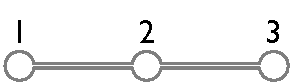
\includegraphics[width=.2\textwidth]{img/sample-1.pdf}

Kui alustada ruumis~$2$ ja külastada ruume järjekorras $2$, $1$, $2$, $3$, siis saab masinad välja
lülitada aegadel $0$ (ruumis $2$), $1$ (ruumis $1$) ja $3$ (ruumis $3$). Nii läheb kokku raisku
$0+1+3=4$~liitrit vedelikku.
Kui aga alustada ruumis~$1$ ja külastada ruume järjekorras $1$, $2$, $3$, siis läheb raisku
$0+1+2=3$~liitrit, mis on eelmisest parem tulemus.

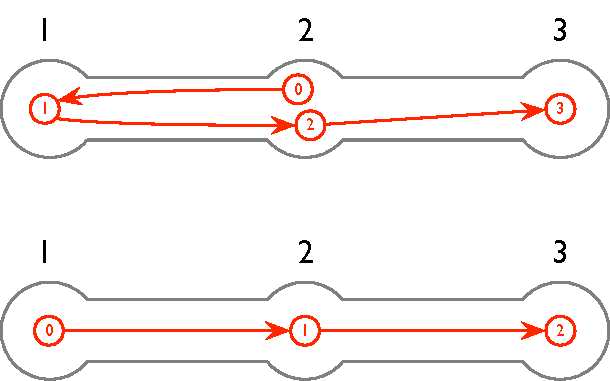
\includegraphics[width=.4\textwidth]{img/sample-1-ans.pdf}

\section*{Sisend}

Sisendi esimesel real on täisarv $n$, ruumide arv.
Eeldame, et ruumid on nummerdatud $1$, $\ldots$, $n$.
Järgmised $n-1$ rida koosnevad igaüks kahest tühikutega eraldatud täisarvust $u$ ja $v$,
kus $1\leq u < v \leq n$, % constraint:hallnames
mis tähendab, et ruumide~$u$ ja $v$ vahel on tunnel.

\section*{Väljund}

Trüki välja üksainus täisarv: vähim võimalik mahaläinud vedeliku kogus liitrites.

\section*{Piirangud ja hindamine}

Alati kehtib
$1\leq n\leq 10^5$. % constraint:n

Selles ülesandes on testid jagatud gruppidesse, iga grupp on väärt mingi arvu punkte.
Iga grupi eest saavad punkte vaid need lahendused, mis läbivad kõik sellesse gruppi kuuluvad testid.
Sinu lõplik skoor on esituste maksimum.

\medskip
\begin{tabular}{lll}
Grupp & Punktid & Lisapiirangud \\\hline
  $1$ & $18$ & ükski ruum ei ole ühendatud rohkema, kui kahe tunneliga\\
  $2$ & $19$ & ülimalt üks ruum on ühendatud rohkema, kui kahe tunneliga\\
  $3$ & $20$ & $n\leq 10$\\
  $4$ & $21$ & $n\leq 1000$\\
  $5$ & $22$ & \emph{Lisapiirangud puuduvad}
\end{tabular}
